\subsection{Testkonzept Hardware}\label{sec:testkonzeptHardware}
Damit ein reibungsloser Betrieb möglich ist, müssen die einzelnen Hardware Komponenten auf Herz und Nieren geprüft werden. Nachfolgend werden die Testverfahren genauer beschrieben und die Testergebnisse aufgelistet.

\subsubsection*{Schutzmechanismen Batterie}\label{sec:batterie}
Die Batterie weist einige Schutzmechanismen auf, welche alle getestet werden müssen. Als erstes wurde der Tiefentladungsschutz geprüft. Um dies zu testen wurde ein Winderstand der Dimension 9$\Omega$ angeschlossen, wobei gemäss Berechnung \ref{eq:Entladestrom} ein Entladestrom von rund 400mA resultierte.

\begin{equation}
\centering
I_{discharge}=\frac{U}{R}=\frac{3.7V}{9\Omega }= 411mA
\label{eq:Entladestrom}
\end{equation}

Während dem Entladevorgang wurde stets die Spannung überwacht, wobei die Spannung von 3.7V auf bis 2.5V absank. Nach dem die 2.5V Schwellenspannung unterschritten wurde, brach der integrierte Batterieschutz die Spannungsversorgung ab. Die Widerstände wurden abgehängt und der gesamte Vorgang wurde kurze Zeit danach mit dem selben Endergebnis wiederholt.
\\
Als nächstes wurde ein Kurzschlusstest durchgeführt, wobei hier der Schwellenstrom gemäss Datenblatt bei 4.8 liegt. Gemäss dem $U=R\cdot I$ Gesetz, wurde ein Widerstand der Grösse von $700m\Omega$ verwendet damit der Grenzwert überschritten wird. Auch bei diesem Versuch, riegelte das PCM den hohen Entladungsstrom ab und schaltete die Versorgungsspannung der Batterie ab.

\subsubsection*{Ladeschaltung der Batterie}\label{sec:batterie}
Für die Ladeschaltung der Batterie wurde (wie bereits im Kapitel \ref{sec:Energiespeicher} Abschnitt Schutzeinrichtungen erwähnt) ein Lade-IC verwendet. Dieser reguliert zuerst die Spannung wobei nach Erreichung des Schwellenwertes von $4.2V$ den Strom auf $0A$ herunter reguliert. Dieser Vorgang wurde während einem gesamten Ladevorgang der Batterie beobachtet und dokumentiert. Hierbei ist wichtig zu erwähnen, dass dieses Testing nicht die induktive Energieübertragung verwendete, sondern der Fokus auf der Funktionalität des Lade-ICs beschränkt und somit das Netzgerät \glqq Power Supply\grqq\space der Firma \glqq K. Witmer\grqq\space als Spannungsspeisung verwendet wurde. Aus diesem Grund ist auch ein Strom von $400mA$ wie auch eine Ladezeit von lediglich rund $270$ Minuten $(\hat{=} 4.5h)$ ersichtlich was die effektiven Ladewerte mittels induktiver Ladung deutlich unterbietet. Die nachfolgende Abbildung \ref{fig:LadekurveLadeIC} zeigt die Regulierung der Spannung (blaue Kurve) wie auch die Regulierung des Stromes (rote Kurve) in Abhängigkeit der Zeit in Minuten.

\begin{figure}[H]
	\begin{center}
		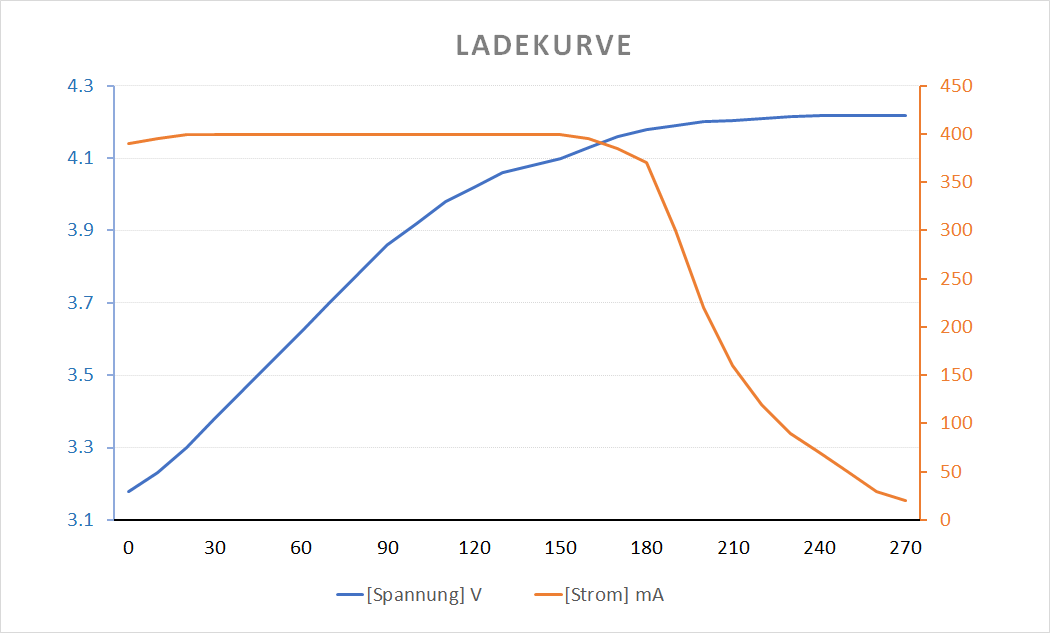
\includegraphics[width=120mm]{data/LadekurveLadeIC.png}
		\caption[Ladekurve Lade-IC]{Ladekurve Lade-IC} %picture caption
		\label{fig:LadekurveLadeIC}
	\end{center}
\end{figure}

Die oben genannten Vorgänge der Spannungs- und Stromregulierung sind in dieser Grafik gut ersichtlich wobei der Ladevorgang nach dem erreichen von rund 20mA als fertig betrachtet wurde.

\subsubsection*{Induktive Ladeschaltung}\label{sec:batterie}
In diesem Abschnitt werden die Ergebnisse der induktiven Ladeschaltung präsentiert. Nachfolgend zeigt Abbildung \ref{fig:InduzierterStrom} die Abhängigkeit zwischen induziertem Strom und Spannung in Abhängigkeit zur Distanz z zwischen den Induktionsspulen.

\begin{figure}[H]
	\begin{center}
		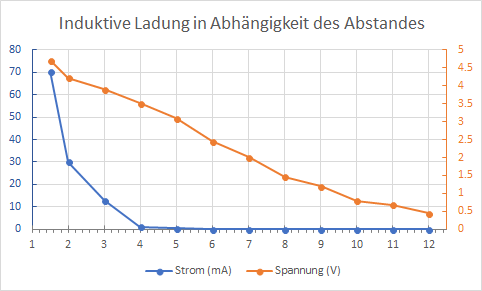
\includegraphics[width=100mm]{data/InduktiveLadung.png}
		\caption[Induzierter Strom in Abhängigkeit der Distanz]{Induzierter Strom in Abhängigkeit der Distanz} %picture caption
		\label{fig:InduzierterStrom}
	\end{center}
\end{figure}

In der Abbildung ist gut sichtbar, dass die Spannung fast linear zur Distanz abnimmt, hingegen der Ladestrom der Batterie extrem schnell klein wird. Aufgrund dieser Erkenntnissen sind wir gezwungen eine möglichst kurze Entfernung zwischen den Spulen einzuhalten weshalb wir eine Ladestation entworfen haben, welche die bestmöglichen Induktionswerte garantiert. Der minimale Abstand welcher beim Ladezyklus erreicht werken kann beträgt rund $1.5mm$. Dieser Abstand entspricht ziemlich genau der Wanddicke des Dōjōs. Bei diesem Abstand resultiert ein an die Batterie gelieferter Strom von $70mA$, wobei eine Ladezeit von $XX$ Stunden resultiert. Diese $XX$ Stunden wurden während einem Laborversuch errechnet, wobei sich dieser in zwei Ladezyklen unterteilt. Beim ersten Ladezyklus wird die Batterie mit konstantem Strom geladen. Dies hat zur Folge, dass die Spannung von ihrem Minimalwert $3.3V$ auf den Schwellenwert von $4.2V$ reguliert wird. Um auf die notwendige Ladezeit des ersten Ladezyklus zu kommen, kann die Zeit während einer beliebig grossen Spannungsdifferenz gestoppt werden. Generell gilt: Umso grösser die Spannungsdifferenz, desto genauer die Approximation. Die Endzeit kann wie in nachfolgender Berechnung \ref{eq:LadezeitSpannungsregelung} linear hochgerechnet werden. 

\begin{equation}
\centering
t_{charge_{1}}=\frac{1.1 V}{(\frac{XX V}{XX Minuten})}=XX Minuten= XX Stunden
\label{eq:LadezeitSpannungsregelung}
\end{equation}

Für die Spannungsregelung sind somit $XX$ Stunden notwendig. Da jedoch der Ladezyklus nach vollständiger Spannungsregelung noch nicht abgeschlossen ist, folgt noch die benötigte Zeit für die Stromregelung. Da diese nicht einfach berechnet werden kann, wurde dieser Prozess im Labor durchgeführt und gestoppt. Es ergab sich hierbei eine Zeit von:
\begin{equation}
\centering
t_{charge_{2}}= XX Stunden
\label{eq:LadezeitStromregelung}
\end{equation}

Der gesamte Ladezyklus ($t_{charge}=t_{charge_{1}}+t_{charge_{2}}$) benötigt somit $XX$ Stunden um die Batterie vollständig aufzuladen.  
